\documentclass[12pt]{article}

% -------------------- preamble --------------------
\usepackage{amsthm}
\newtheorem*{exercise}{Exercise}
\newtheorem*{solution}{Solution}
\usepackage{amsmath, amssymb}
\usepackage{physics}
\usepackage{geometry}
\usepackage{hyperref}
\usepackage{nicematrix}
\usepackage{empheq}
\usepackage{xcolor}
\usepackage{tikz}
\usepackage{pgfplots}
\usepackage{wrapfig}
\usepackage{cancel}
\usetikzlibrary{positioning, angles, quotes}
\usetikzlibrary{shapes.geometric}

\newcommand*\widefbox[1]{\fbox{\hspace{2em}#1\hspace{2em}}}

\geometry{margin=1in}

\title{Lecture Notes: Relativity\\
\large Based on Youtube series by eigenchris}
\author{}
\date{}

% -------------------- document --------------------
\begin{document}
\maketitle
\tableofcontents
\newpage

% -------------------- input sections --------------------
\section{Introduction to Relativity}

Before we even start by exploring relativity, either it being Gelilean or Eistein one, we should ask ourselves: what is relativity?\\

\textbf{Relativity is how the laws of motion work in different reference frames}.

\subsection{Gelilean Relativity}
Now, the Galilean principle of relativity, states that \textbf{the laws of motion are the same in all inertial frames of reference.}\\

And an inertial reference frame, is a reference frame that's not accelerating.\\

If we think about a very simple experiment from a scientist dropping a ball on the floor in his office room, and a car passing by this office and observing the experiment:

\begin{itemize}
    \item The scientist will just see the ball falling down straight to the ground
    \item A potential car passing (at a constant velocity) by the office and looking at it, will see the ball moving along a curved trajectory towards the floor
\end{itemize}

At the end, they would disagree on the velocity, on the momentum, kinetic energy as well.\\
So like, what are they actually agreeing on? Well, they would agree on:

\begin{itemize}
    \item The time passed
    \item The size of the ball
    \item The mass of the ball
\end{itemize}

Eventually, this leads to them agreeing on the laws of motion, the Newton's three laws of motion and the gravitational law:

\begin{equation}
    \color{red}\vec{F} = m \vec{a}
\end{equation}
\begin{equation}
\color{blue}\vec{F} = G \frac{m_1 m_2}{r^2}(-\hat{r})
\end{equation}

And if we copy the experiment of dropping the ball inside the car passing by at constant velocity, the experiment 
will be exactly the same as the scientist run in his own office.\\
So the laws of motion are exactly the same in all inertial reference frames.

\textbf{There's no experiment you can do to determine if your reference frame is stationary, or moving at constant speed. And there's no special reference frame truly stationary}\\

And what would instead be an example of non-inertial reference frame? Well an elevator accelerating, or a car 
accelerating forward, a car turning a corner.\\
And in all these non-inertial situations, the passenger (man in the elevator, or driver in the car) always feels a misterious fictitious force 
pulling them in the opposite direction of the acceleration.
\textbf{This means that a passenger in an accelerating reference frame, will have different set of laws of motion!}
Everytime they use Newton's second law, they need to add an extra term for the fictitious force in order to predict the motion
of objects correctly.\\

\subsection{Special Relativity}

This type of relativity is the one we experience when moving to speed close to the speed of light.\\

The story starts in the 19th centuryt with Maxwell's equations of electro-magnetism:

\begin{align*}
    \nabla \cdot \vec{E} &= \rho\\
    \nabla \times \vec{E} &= -\frac{\partial \vec{B}}{\partial t}\\
    \nabla \vec{B} &= 0\\
    \nabla \times \vec{B} &= \mu_0 \vec{J} + \mu_0 \epsilon_0 \frac{\partial \vec{E}}{\partial t}
\end{align*}

There's a problem with these equations, when we combine them together, we obrain
equations for electromagnetic waves, or in other words..light.\\

\begin{align*}
    \nabla^2\vec{E} = \frac{1}{c^2}\left(\frac{\partial^2 \vec{E}}{\partial^2t}\right)&&
    \nabla^2\vec{B} = \frac{1}{c^2}\left(\frac{\partial^2 \vec{B}}{\partial^2t}\right)
\end{align*}

These equations say that light, in a vacuum, travels at the speed of $c = \frac{1}{\sqrt{\mu_0 \epsilon_0}}$, and this 
speed, if you plug in the two constants for the megnetic permability $\mu_0 = 4\pi \times 10^{-7} H/m$, and electric permittivity $\epsilon_0 = 8.854 \times 10^{-12} F/m$, is equal to
$c \approx 3 \times 10^8 m/s$.\\

If you think about this, and try to correlate to other speeds, like the speed of sound, you know that that's measured relative to air, or the speed of 
ocean's waves, that's relative to water, etc., but then what's the speed of light relative to, if it travels in the vacuum?
Remember that the Galilean relativity states that there's no special reference frame! And all motion is always relative to something else.\\

So what are we measuring the speed of light relative to in the vacuum, if the vacuum is just empty space??
To get around this problem, scientists predicted the existence of the "aether", a special stationary reference frame that light travels in.
But experiments such as the "Michelson-Morley" one showed that aether does not exist.\\

And this is where Einstein comes in, proposing that the speed of light $c$ is the same in all reference frames, basically 
treating the speed of light as a law of physics.
So in an attempt to build a new theory of relativity, Einstein began by agreeing with Galileo and said that the laws of motion are the 
same in all inertial reference frames, but he expanded this principle by including the Maxwell's equations in the laws of motion that the reference frames 
agree upon, and made the speed of light as a constant that everyone agree upon.\\

Finally, the two Einstein postulates of Special Relativity are:

\begin{itemize}
    \item Laws of physics are the same in all inertial reference frames;
    \item Speed of light in a vacuum $c$ is equal for all observers in inertial reference frames (a.k.a speed of light in a vacuum is included in laws of physics).
\end{itemize}

Unfortunately, these postulates are not compatible with the Galilean relativity!
To see why, we can simply think about a similar experiment we thought about above, a scientist on the ground, and a 
car passing by at constant velocity $v$ to the right, but this time with a giant flash light attached on its roof.\\

In the car's frame, the driver sees the scientist pass by with a speed of $v$ to the left, and the light coming out from the flash light
traveling to the right at speed $c$.
But in the frame of the scientist, since the car is traveling right with speed $v$, the light coming out of the flash light, would appear to have 
the speed of light $c$, plus the car speed $v$, and this violates the postulate that the speed of light is equal to all inertial frames observers.\\

The only way to fix this, is to take time and space, which Galilean relativity stated as pointf of agreement among observers in different inertial reference frames, 
and change them from things that everyone agrees on, to things that everyone can disagree on.\\
In the theory of special relativity, time and space become relative and depend on the observer's reference frame, just like the velocity, momentum and kinetic energy.\\

To understand this, let's consider the example of a train passing by a station at constant speed $v$, this speed is measured relative to the platform
on the ground where a scientist is standing. And now let's see how a beam of light behave on the train.\\

Imagine inside the train, a beam of light sent from one of the vagon's floors, towards the roof parpendicular to the train travel direction, and on the roof there's a mirror reflecting the light back to the floor.
The distance between the floor and roof of the vagon is $d$.

We can use the time it takes to travel this distance as a kind of clock, so instead of ticking once per second, this clock will tick once every time tha beam
crosses the train vagon in one direction. This would be given by:

\begin{equation}
    \begingroup\color{teal}\Delta t\endgroup = \frac{d}{c}
\end{equation}

Now consider this from the point of reference of the scientist on the platform ground.\\
Since the train is passing by at speed $v$ on the right, he sees the beam of light traveling in a triangle
shape because of the train motion.

\begin{center}
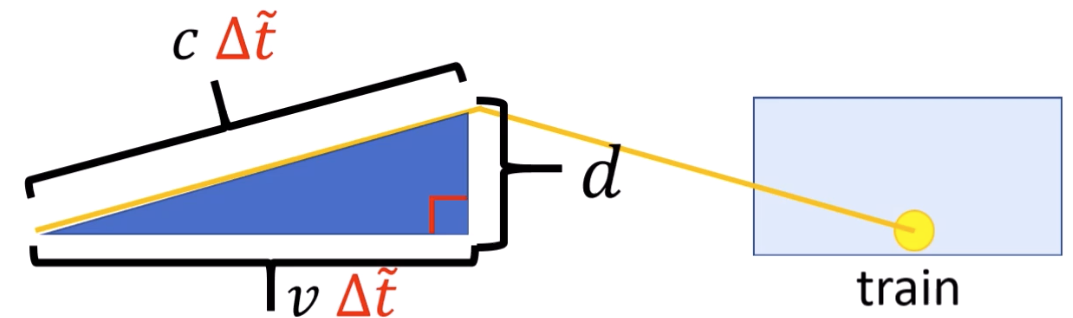
\includegraphics[scale=0.3]{figures/train-lorentz.png}
\end{center}

So in the frame of the platform, the light takes $\color{red}\Delta\tilde{t}$ time to cross the train:

\begin{align*}
    d^2 + \left(v \begingroup\color{red}\Delta\tilde{t}\endgroup\right)^2 &= \left(c \begingroup\color{red}\Delta\tilde{t}\endgroup\right)^2\\
    \frac{d^2}{c^2} + \frac{v^2}{c^2}\left(\begingroup\color{red}\Delta\tilde{t}\endgroup\right)^2 &= \left(\begingroup\color{red}\Delta\tilde{t}\endgroup\right)^2\\
    \frac{d^2}{c^2} &= \left(\begingroup\color{red}\Delta\tilde{t}\endgroup\right)^2 \left(1-\frac{v^2}{c^2}\right)
\end{align*}

which means that:

\begin{align*}
    \left(\begingroup\color{teal}\Delta t\endgroup\right)^2 &= \left(\begingroup\color{red}\Delta\tilde{t}\endgroup\right)^2 \left(1-\frac{v^2}{c^2}\right)\\
    \begingroup\color{red}\Delta\tilde{t}\endgroup &= \begingroup\color{teal}\Delta t\endgroup \left(\frac{1}{\sqrt{1-\frac{v^2}{c^2}}}\right) = \begingroup\color{teal}\Delta t\endgroup \gamma_v
\end{align*}

This factor that you see, it's called the Lorentz factor, and we often write it as $\gamma_v$.\\

This tells us that, the time calculated by the scientist on the ground platform $\color{red}\Delta\tilde{t}$ is actually greater 
than the time calculated by the moving train $\color{teal}\Delta t$.\\
In other words, the travel time for the light beam in each reference frame is not equal. When we measure the time between clock ticks for a moving 
clock, and measure the time between clock ticks for a stationary clock, we find that the time between clock ticks for the moving clock is larger.\\
This effect is called time dilation.\\

There is a similar effect called length contraction, where rods that are moving appear to have a shorter length than the same 
rods when they are standing still. However length contraction only happens along the direction of motion, in the direction perpendicular to motion, no length contraction happens.

\begin{equation}
    \begingroup\color{red}\Delta\tilde{l}\endgroup = \begingroup\color{teal}\Delta l\endgroup \frac{1}{\gamma_v}
\end{equation}

These effects are obviously only visible and noticeable when the speed is close to the speed of light, otherwise
the Lorentz factor is practically one.\\

As an example, one experiment showing the time dilation is the Rossi-Hall one performed in 1941, on the muon lifetime.
Muons are subatomic charged particles created in Earth's atmosphere by cosmic rays from outer space.\\
Liek electrons, muons are negatively charged, but unlike electrons, they're very unstable and decay on average, in $2.2 \mu s$.
Without considering special relativity effects, a muon would traveling at $0.995c$ would reach $656m$ on average before it decays.
But this would not be enough time for a muon to reach earth from atmosphere.\\
At this speed, the Lorentz factor ends up being around 10, so taking now account for the time delation effect, a traveling muon will live
for 10 times longer than expected lifetime from the stationary earth observer.\\
So this means that the muon would travel about 6.5km on average before it decays, which is indeed
enough to reach the surface of our planet from the atmosphere.\\

If the muon is even faster, time dilation effect would be even larger, which means that the muons can travel further distances, even underground possibly.
The fact that we see muons reaching Earth's surface is a real physical evidence that special relativity is correct. 

Now, one last thing...\\
Have you ever wondered why this is called \textbf{special} relativity in the first place?
Well this theory has a big problem, and that is, that's not consistent with Newtonian Gravity. If we think about a line of planets, each exerciting its force on 
an astronaut, according to Newton's law of gravity, the astronaut will experience a force upward by the total net force.

\begin{center}
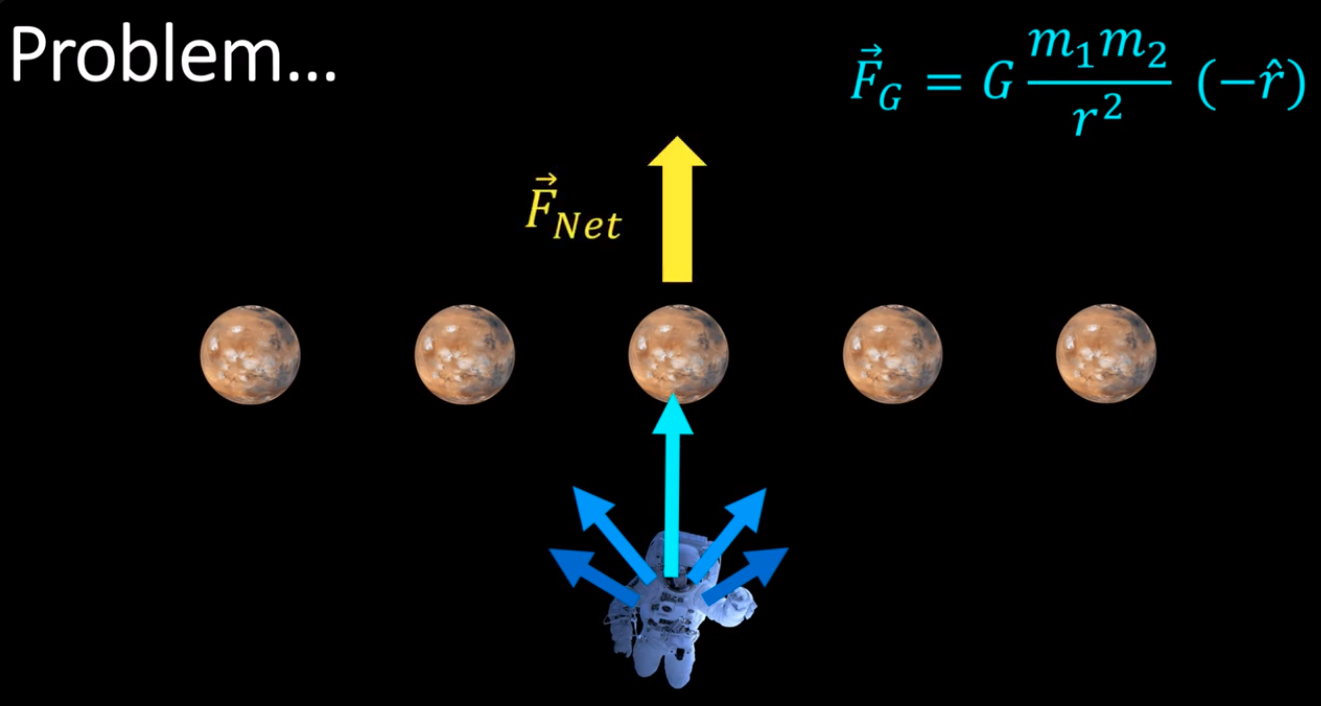
\includegraphics[scale=0.2]{figures/astronaut-issue-01.png}
\end{center}

But if looked from a different reference frame, moving at velocity $v$ parallel to the planets' line, these planets 
unergo length contraction along the line, so those become more densely packed together, and this would increase the gravitational net force 
on the astronaut:

\begin{center}
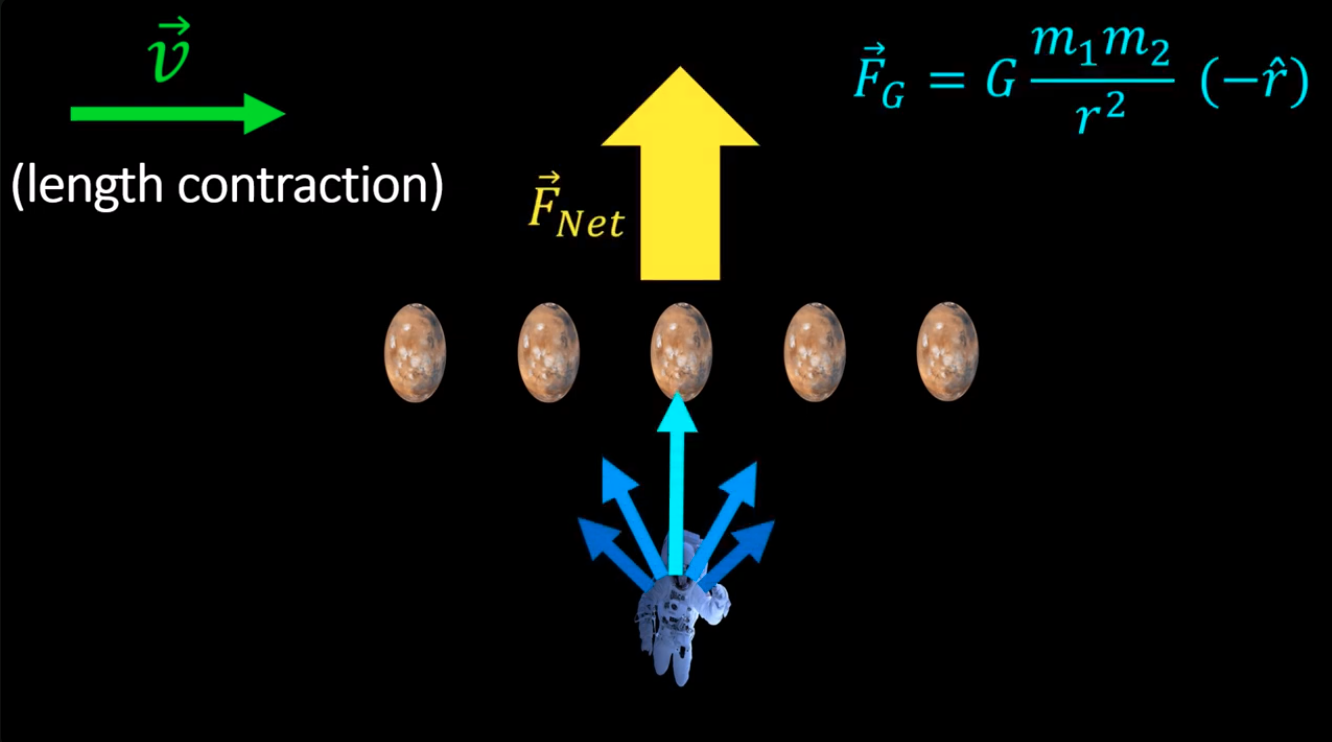
\includegraphics[scale=0.2]{figures/astronaut-issue-02.png}
\end{center}

The fact that the gravitational force is different in different reference frames, means that the Newton's law of gravity is not obeyed, hence
the inconsistency with special relativity.\\

To get this right, we need a new theory of relavitiy that deals with gravity properly, which is General Relativity.
End of the story is that, special relativity is valid assuming litte or no gravity, that's why it's called special. It's a special case of no gravity.


% -------------------- bibliography --------------------
\begin{thebibliography}{9}
\bibitem{eigenchris}
eigenchris, \textit{Relativity}, YouTube video series,\\
\url{https://www.youtube.com/playlist?list=PLJHszsWbB6hqlw73QjgZcFh4DrkQLSCQa}
\end{thebibliography}

\end{document}
